\documentclass{article}
\usepackage[utf8]{inputenc}
% are all of these packages really necessary?
% no.
% i'm just too lazy to only grab the packages i want for a specific
% document, so i just glob all of my most commonly used packages together
% this is bad practice.
\usepackage{amsmath,amsthm,amssymb,amsfonts, fancyhdr, color, comment, graphicx, environ, mdframed, soul, calc, enumitem, mdframed, xcolor, geometry, empheq, mathtools, tikz, pgfplots}

\usetikzlibrary{external}
\tikzexternalize[prefix=tikz/,optimize command away=\includepdf]

%tikzpicture
\usepackage{tikz}
\usepackage{scalerel}
\usepackage{pict2e}
\usepackage{tkz-euclide}
\usetikzlibrary{calc}
\usetikzlibrary{patterns,arrows.meta}
\usetikzlibrary{shadows}
\usetikzlibrary{external}

%pgfplots
\usepackage{pgfplots}
\pgfplotsset{compat=newest}
\usepgfplotslibrary{statistics}
\usepgfplotslibrary{fillbetween}
\usepgfplotslibrary{polar}

\tikzset{external/export=true}
\pgfplotsset{
    standard/.style={
    axis line style = thick,
    trig format=rad,
    enlargelimits,
    axis x line=middle,
    axis y line=middle,
    enlarge x limits=0.15,
    enlarge y limits=0.15,
    every axis x label/.style={at={(current axis.right of origin)},anchor=north west},
    every axis y label/.style={at={(current axis.above origin)},anchor=south east}
    }
}
\newcommand*\widefbox[1]{\fbox{\hspace{2em}#1\hspace{2em}}}
% Command "alignedbox{}{}" for a box within an align environment
% Source: http://www.latex-community.org/forum/viewtopic.php?f=46&t=8144
\newlength\dlf  % Define a new measure, dlf
\newcommand\alignedbox[2]{
% Argument #1 = before & if there were no box (lhs)
% Argument #2 = after & if there were no box (rhs)
&  % Alignment sign of the line
{
\settowidth\dlf{$\displaystyle #1$}  
    % The width of \dlf is the width of the lhs, with a displaystyle font
\addtolength\dlf{\fboxsep+\fboxrule}  
    % Add to it the distance to the box, and the width of the line of the box
\hspace{-\dlf}  
    % Move everything dlf units to the left, so that & #1 #2 is aligned under #1 & #2
\boxed{#1 #2}
    % Put a box around lhs and rhs
}
}

\newcommand{\lrp}[1]{\left( #1 \right)}
\newcommand{\abs}[1]{\left\vert #1 \right\vert}
\newcommand{\lra}[1]{\left\langle #1 \right\rangle}
\newcommand{\lrb}[1]{\left[ #1 \right]}
\newcommand{\iintR}[0]{\iint\limits_{R}}

\geometry{letterpaper, portrait, margin=1in}
\renewcommand{\footrulewidth}{0.8pt}
\setlength\parindent{0pt}
\pagestyle{fancy}
\lhead{Christina Phan}
\rhead{MAT 21D} 
\chead{\textbf{Homework 3 Solutions}}

\newcommand{\Solution}{\textit{Solution}}
 \pgfplotsset{compat=1.18}
\begin{document}
\textbf{Problem 1}

Evaluate the integral by converting to polar coordinates.

\textbf{(a)} $\displaystyle\int_0^2\int_0^{\sqrt{4-y^2}}x^2+y^2\,dx\,dy$

\Solution

It's a good idea to graph the Cartesian region to see how it would relate to the polar region. That is, graph $y=0$, $y=2$, $x=0$, and $x=\sqrt{4-y^2}$.
\begin{center}
\resizebox{3.5cm}{!}{
    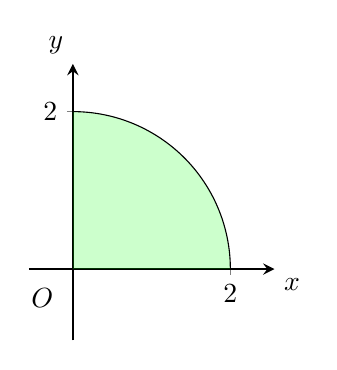
\begin{tikzpicture}
    \begin{axis}[standard,
            xtick={2},
            ytick={2},
            samples=1000,
            xlabel={$x$},
            ylabel={$y$},
            xmin=-.2,xmax=2.2,
            ymin=-0.5,ymax=2.2,
            x=1cm,
            y=1cm/1,
           ]
\node[anchor=center,label=south west:$O$] at (axis cs:0,0){};
\addplot[name path=F,domain={0:2}]{sqrt(4-x^2)};
\addplot[name path=G, domain={0:2}]{0};
\addplot[fill=green, fill opacity=0.2] fill between [of=F and G, soft clip={domain=0:2}];
    \end{axis}
    \end{tikzpicture}
}
\end{center}
Based on the graph, it looks like our angle $\theta$ is between $0$ and $\displaystyle\frac{\pi}{2}$.

The lower bound of $r$ is clearly $0$. We can get the upper bound of $r$ quite easily as well from the function $x=\sqrt{4-y^2}$.
\begin{align*}
    x&=\sqrt{4-y^2}\\
    x^2&=4-y^2\\
    x^2+y^2&=4\\
    r^2&=4\tag{in polar, $x^2+y^2=r^2$}\\
    r&=2\tag{keep positive $r$}
\end{align*}
Now, we can translate our Cartesian integral into its equivalent polar integral.
\begin{align*}
\int_0^2\int_0^{\sqrt{4-y^2}}x^2+y^2\,dx\,dy&=\int_0^{\frac{\pi}{2}}\int_0^{2}(r^2)r\,dr\,d\theta\tag{in polar, $x^2+y^2=r^2$}\\
&=\int_0^{\frac{\pi}{2}}\lrb{\frac{1}{4}r^4}_0^2\,d\theta\\
&=\int_0^{\frac{\pi}{2}}4\,d\theta\\
&=\lrb{4\theta}_0^{\frac{\pi}{2}}\\
&=\boxed{2\pi}
\end{align*}
\textbf{(b)} $\displaystyle\int_0^6\int_0^yx\,dx\,dy$

\Solution

It's a good idea to graph the Cartesian region to see how it would relate to the polar region. That is, graph $y=0$, $y=6$, $x=0$, and $x=y$.
\begin{center}
\resizebox{3.5cm}{!}{
    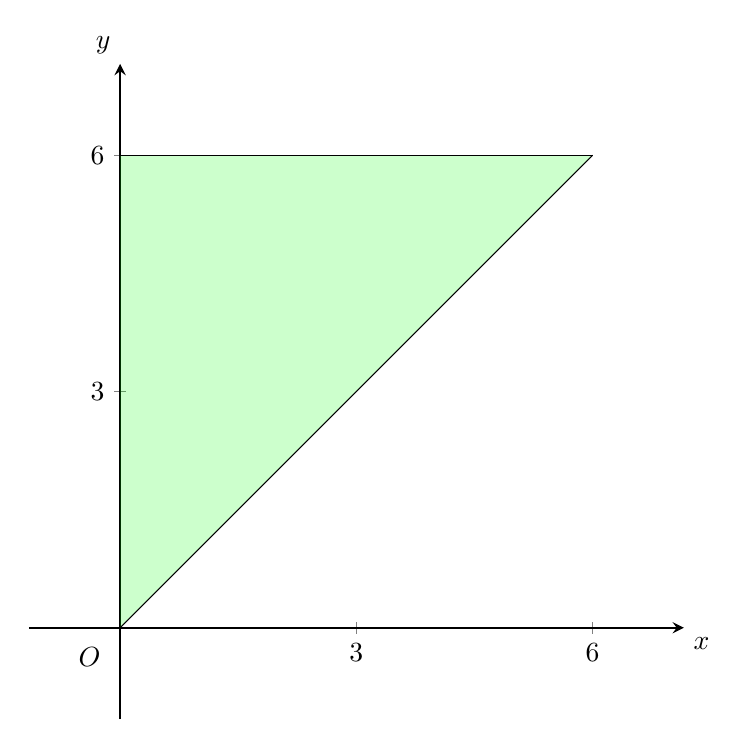
\begin{tikzpicture}
    \begin{axis}[standard,
            xtick={3, 6},
            ytick={3, 6},
            samples=1000,
            xlabel={$x$},
            ylabel={$y$},
            xmin=-0.2,xmax=6.2,
            ymin=-0.2,ymax=6.2,
            x=1cm,
            y=1cm/1,
           ]
\node[anchor=center,label=south west:$O$] at (axis cs:0,0){};
\addplot[name path=F,domain={0:6}]{x};
\addplot[name path=G,domain={0:6}]{6};
\addplot[fill=green, fill opacity=0.2] fill between [of=F and G, soft clip={domain=0:6}];
    \end{axis}
    \end{tikzpicture}
}
\end{center}
The upper bound of $\theta$ is $\displaystyle\frac{\pi}{2}$. To get the lower bound of $\theta$ we can use the line $x=y$.
\begin{align*}
    x&\geq y\\
    \frac{x}{y}&\geq 1\\
    \tan \theta &\geq 1\\
    \theta & \geq \tan^{-1} 1\\
    \theta & \geq \frac{\pi}{4}
\end{align*}
Our lower bound of $r$ is clearly $0$. To get our upper bound of $r$, we can use the line $y=6$.
\begin{align*}
    y &\leq 6\\
    r\sin \theta &\leq 6\tag{in polar, $y=\sin\theta$}\\
    r &\leq 6\csc \theta \tag{$\displaystyle \frac{1}{\sin\theta}=\csc\theta$}
\end{align*}
Now, we can translate our Cartesian integral into its equivalent polar integral.
\begin{align*}
    \int_0^6\int_0^yx\,dx\,dy&=\int_{\frac{\pi}{4}}^{\frac{\pi}{2}}\int_0^{6\csc\theta}( r\cos \theta)r\,dr\,d\theta\tag{in polar, $x=r\cos\theta$}\\
    &=\int_{\frac{\pi}{4}}^{\frac{\pi}{2}}\int_0^{6\csc\theta} r^2\cos\theta
    \,dr\,d\theta\\
    &=\int_{\frac{\pi}{4}}^{\frac{\pi}{2}}\lrb{\frac{1}{3}r^3\cos\theta}_0^{6\csc\theta}\,d\theta\\
    &=\int_{\frac{\pi}{4}}^{\frac{\pi}{2}} 72 \csc^3\theta \cos\theta \,d\theta\\
    &=72\int_{\frac{\pi}{4}}^{\frac{\pi}{2}} \csc^2\theta\cot\theta\,d\theta\tag{$\displaystyle\csc\theta\cos\theta=\frac{\cos\theta}{\sin\theta}=\cot\theta$}\\
    &u=\cot\theta \hspace{2em}du-\csc^2\theta\,d\theta\\
    &u\lrp{\frac{\pi}{4}}=1\hspace{2em}u\lrp{\frac{\pi}{2}}=0\\
    &=-72\int_1^{0}u\,du\\
    &=72\int_0^1u\,du\\
    &=72\lrb{\frac{1}{2}u^2}_0^1\\
    &=\boxed{36}
\end{align*}
\textbf{(c)} $\displaystyle \int_1^{\sqrt{3}}\int_1^x\,dy\,dx$

\Solution

It's a good idea to graph the Cartesian region to see how it would relate to the polar region. That is, graph $x=1$, $x=\sqrt{3}$, $y=1$, and $y=x$. 
\begin{center}
\resizebox{3.5cm}{!}{
    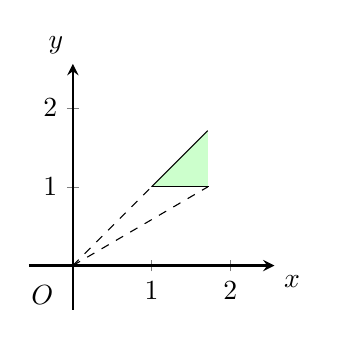
\begin{tikzpicture}
    \begin{axis}[standard,
            xtick={1,2},
            ytick={1,2},
            samples=1000,
            xlabel={$x$},
            ylabel={$y$},
            xmin=-0.2,xmax=2.2,
            ymin=-.2,ymax=2.2,
            x=1cm,
            y=1cm/1,
           ]
\node[anchor=center,label=south west:$O$] at (axis cs:0,0){};
\addplot[name path=F,domain={1:1.713}]{x};
\addplot[name path=G,domain={1:1.713}]{1};
\addplot[dashed, domain={0:1.713}]{0.583*x};
\addplot[dashed, domain={0:1}]{x};
\addplot[fill=green, fill opacity=0.2] fill between [of=F and G, soft clip={domain=1:1.713}];
    \end{axis}
    \end{tikzpicture}
}
\end{center}
The dashed lines are there to help us figure out what $\theta$ and $r$ are. They are not necessary.

For our lower bound of $\theta$, we can get it from the point $\displaystyle \lrp{\sqrt{3}, 1}$.
\begin{align*}
    \frac{y}{x}&=\tan \theta\\
\frac{1}{\sqrt{3}}&=\tan \theta \\
\theta &= \tan^{-1}\frac{1}{\sqrt{3}}\\
\theta &= \frac{\pi}{6}
\end{align*}
For our upper bound of $\theta$, we can get it from the line $y=x$.
\begin{align*}
    y&=x\\
    r\sin \theta &= r\cos\theta\\
    \frac{r\sin\theta}{r\cos\theta} &= 1\\
    \tan \theta &= 1\\
    \theta &= \tan^{-1}1\\
    \theta &= \frac{\pi}{4}
\end{align*}
For our lower bound of $r$, we can get it from the line $y=1$.
\begin{align*}
    y&=1\\
    r\sin\theta&=1\tag{in polar, $y=r\sin\theta$}\\
    r&=\csc\theta\tag{$\dfrac{1}{\sin\theta}=\csc\theta$}
\end{align*}
For our upper bound of $r$, we can get it from the line $x=\sqrt{3}$.
\begin{align*}
    x&=\sqrt{3}\\
    r\cos\theta&=\sqrt{3}\tag{in polar, $x=r\cos\theta$}\\
    r&=\sqrt{3}\sec\theta\tag{$\dfrac{1}{\cos\theta}=\sec\theta$}
\end{align*}
Now, we can translate our Cartesian integral into its equivalent polar integral.
\begin{align*}
    \int_1^{\sqrt{3}}\int_1^x\,dy\,dx&=\int_{\frac{\pi}{6}}^{\frac{\pi}{4}}\int_{\csc\theta}^{\sqrt{3}\sec\theta}r\,dr\,d\theta\\
    &=\int_{\frac{\pi}{6}}^{\frac{\pi}{4}}\lrb{\frac{1}{2}r^2}_{\csc\theta}^{\sqrt{3}\sec\theta}\,d\theta\\
    &=\int_{\frac{\pi}{6}}^{\frac{\pi}{4}} \frac{3}{2}\sec^2\theta -\frac{1}{2}\csc^2\theta\,d\theta\\
    &=\lrb{\frac{3}{2}\tan\theta+\frac{1}{2}\cot\theta}_{\frac{\pi}{6}}^{\frac{\pi}{4}}\\
    &=\lrp{\frac{3}{2}+\frac{1}{2}}-\lrp{\frac{3}{2}\lrp{\frac{1}{\sqrt{3}}}+\frac{1}{2}\lrp{\sqrt{3}}}\\
    &=\boxed{2-\sqrt{3}}
\end{align*}
\textbf{(d)} $\displaystyle \int_0^{1}\int_{-\sqrt{1-y^2}}^{\sqrt{1-y^2}}3y\,dx\,dy$

\Solution

It's a good idea to graph the Cartesian region to see how it would relate to the polar region. That is, graph $y=0$, $y=1$, $x=-\sqrt{1-y^2}$, and $x=\sqrt{1-y^2}$.
\begin{center}
\resizebox{3.5cm}{!}{
    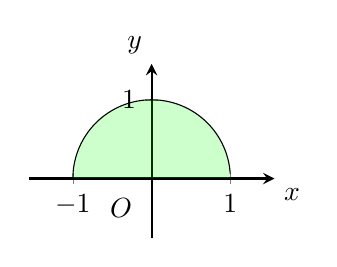
\begin{tikzpicture}
    \begin{axis}[standard,
            xtick={-1, 1},
            ytick={1},
            samples=1000,
            xlabel={$x$},
            ylabel={$y$},
            xmin=-1.2,xmax=1.2,
            ymin=-.5,ymax=1.2,
            x=1cm,
            y=1cm/1,
           ]
\node[anchor=center,label=south west:$O$] at (axis cs:0,0){};
\addplot[name path=F,domain={-1:1}]{sqrt(1-x^2)};
\addplot[name path=G,domain={-1:1}]{0};
\addplot[fill=green, fill opacity=0.2] fill between [of=F and G, soft clip={domain=-1:1}];
    \end{axis}
    \end{tikzpicture}
}
\end{center}
Based on the graph, it looks like our angle $\theta$ is between $0$ and $\pi$.

The lower bound of $r$ is clearly $0$. We can get the upper bound of $r$ quite easily as well from function $x=\sqrt{1-y^2}$ (just one of the is fine).
\begin{align*}
    x&=\sqrt{1-y^2}\\
    x^2&=1-y^2\\
    x^2+y^2&=1\\
    r^2&=1\tag{in polar, $x^2+y^2=r^2$}\\
    r&=1\tag{keep positive $r$}
\end{align*}
Now, we can translate our Cartesian integral into its equivalent polar integral.
\begin{align*}
\int_0^{1}\int_{-\sqrt{1-y^2}}^{\sqrt{1-y^2}}3y\,dx\,dy&=\int_0^\pi\int_0^1 (3r\sin\theta)r\,dr\,d\theta\tag{in polar, $y=r\sin\theta$}\\
&=\int_0^\pi \int_0^1 3r^2\sin\theta\,dr\,d\theta\\
&=\int_0^\pi \lrb{r^3\sin\theta}_0^1\,d\theta\\
&=\int_0^\pi \sin\theta \,d\theta\\
&=\lrb{-\cos\theta}_0^\pi\\
&=(1)-(-1)\\
&=\boxed{2}
\end{align*}
\textbf{(e)} $\displaystyle \int_0^{\ln 2}\int_0^{\sqrt{(\ln 2)^2-y^2}}e^{\sqrt{x^2+y^2}}\,dx\,dy$

\Solution

It's a good idea to graph the Cartesian region to see how it would relate to the polar region. That is, graph $y=0$, $y=\ln 2$, and $x=0$, and $x=\sqrt{(\ln 2)^2-y^2}$. It looks scary to graph, but don't worry. Just treat the $\ln 2$ like a regular old constant. 
\begin{center}
\resizebox{3.5cm}{!}{
    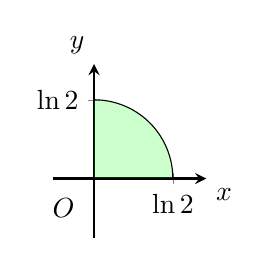
\begin{tikzpicture}
    \begin{axis}[standard,
            xtick={ 1},
            ytick={1},
            samples=1000,
            xlabel={$x$},
            ylabel={$y$},
            xmin=-.3,xmax=1.2,
            ymin=-.5,ymax=1.2,
            x=1cm,
            y=1cm/1,
            xticklabels={ $\ln 2$},
            yticklabels={$\ln 2$}
           ]
\node[anchor=center,label=south west:$O$] at (axis cs:0,0){};
\addplot[name path=F,domain={0:1}]{sqrt(1-x^2)};
\addplot[name path=G,domain={0:1}]{0};
\addplot[fill=green, fill opacity=0.2] fill between [of=F and G, soft clip={domain=0:1}];
    \end{axis}
    \end{tikzpicture}
}
\end{center}
Based on the graph, it looks like our angle $\theta$ is between $0$ and $\dfrac{\pi}{2}$.

The lower bound of $r$ is clearly $0$. We can get the upper bound of $r$ quite easily as well from function $x=\sqrt{(\ln 2)^2-y^2}$.
\begin{align*}
    x&=\sqrt{(\ln 2)^2-y^2}\\
    x^2&=(\ln 2)^2-y^2\\
    x^2+y^2&=(\ln 2)^2\\
    r^2&=(\ln 2)^2\tag{in polar, $x^2+y^2=r^2$}\\
    r&=\ln 2\tag{keep positive $r$}
\end{align*}
Now, we can translate our Cartesian integral into its equivalent polar integral.
\begin{align*}
    \int_0^{\ln 2}\int_0^{\sqrt{(\ln 2)^2-y^2}}e^{\sqrt{x^2+y^2}}\,dx\,dy&=\int_0^{\frac{\pi}{2}}\int_0^{\ln 2} (e^{r})r\,dr\,d\theta\tag{in polar, $x^2+y^2=r^2$}\\
    &u = r \hspace{2em} dv = e^r\,dr\\
    &du=dr \hspace{2em} v = e^r\\
    &=\int_0^{\frac{\pi}{2}} \lrp{\lrb{re^r}_0^{\ln 2}-\int_0^{\ln 2}e^r\,dr}\,d\theta\\
    &=\int_0^{\frac{\pi}{2}}\lrp{ 2\ln 2 -\lrb{e^r}_0^{\ln 2}}\,d\theta\\
    &=\int_0^{\frac{\pi}{2}}2\ln 2 - 1\,d\theta\\
    &=\lrb{(2\ln 2) \theta - \theta}_0^{\frac{\pi}{2}}\\
    &= \boxed{(\ln 2)\pi -\frac{\pi}{2}}
\end{align*}
\textbf{(f)} $\displaystyle \int_{\sqrt{2}}^2\int_{\sqrt{4-y^2}}^y\,dx\,dy$

\Solution

It's a good idea to graph the Cartesian region to see how it would relate to the polar region. That is, graph $y=\sqrt{2}$, $y=2$, $x=\sqrt{4-y^2}$, and $x=y$.
\begin{center}
\resizebox{3.5cm}{!}{
    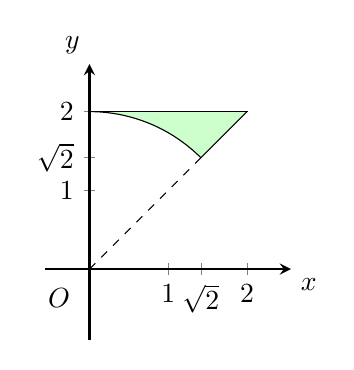
\begin{tikzpicture}
    \begin{axis}[standard,
            xtick={1,1.414,2},
            ytick={1,1.414,2},
            samples=1000,
            xlabel={$x$},
            ylabel={$y$},
            xmin=-0.2,xmax=2.2,
            ymin=-.5,ymax=2.2,
            x=1cm,
            y=1cm/1,
            xticklabels={$1$,$\sqrt{2}$, $2$},
            yticklabels={$1$,$\sqrt{2}$, $2$}
           ]
\node[anchor=center,label=south west:$O$] at (axis cs:0,0){};
\addplot[name path=F,domain={0:2}]{2};
\addplot[name path=G,domain={0:1.414}]{sqrt(4-x^2)};
\addplot[name path=H,domain={1.414:2}]{x};
\addplot[dashed,domain={0:1.414}]{x};
\addplot[fill=green, fill opacity=0.2] fill between [of=F and G, soft clip={domain=0:1.414}];
\addplot[fill=green, fill opacity=0.2] fill between [of=F and H, soft clip={domain=1.414:2}];
    \end{axis}
    \end{tikzpicture}
}
\end{center}
The dashed line is there to help us figure out what $\theta$ and $r$ are. They are not necessary. 

The upper bound of $\theta$ is $\dfrac{\pi}{2}$.

We can get the lower bound of $\theta$ from the line $x=y$.
\begin{align*}
    x&=y\\
    1&=\frac{y}{x}\\
    1&=\tan\theta\tag{in polar, $\displaystyle \frac{y}{x}=\tan\theta$}\\
    \theta &= \tan^{-1}1\\
    \theta &= \frac{\pi}{4}
\end{align*}
We can get the upper bound of $r$ from the line $y=2$.
\begin{align*}
    y&=2\\
    r\sin\theta&=2\tag{in polar, $y=r\sin\theta$}\\
    r&=2\csc\theta\tag{$\dfrac{1}{\sin\theta}=\csc\theta$}
\end{align*}
We can get the lower bound of $r$ from  the curve $x=\sqrt{4-y^2}$.
\begin{align*}
    x&=\sqrt{4-y^2}\\
    x^2&=4-y^2\\
    x^2+y^2&=4\\
    r^2&=4\tag{in polar, $x^2+y^2=r^2$}\\
    r&=2\tag{keep positive $r$}
\end{align*}
Now, we can translate our Cartesian integral into its equivalent polar integral.
\begin{align*}
    \int_{\sqrt{2}}^2\int_{\sqrt{4-y^2}}^y\,dx\,dy&=\int_{\frac{\pi}{4}}^{\frac{\pi}{2}}\int_2^{2\csc\theta}r\,dr\,d\theta\\
    &=\int_{\frac{\pi}{4}}^{\frac{\pi}{2}}\lrb{\frac{1}{2}r^2}_2^{2\csc\theta}\,d\theta\\
    &=\int_{\frac{\pi}{4}}^{\frac{\pi}{2}}2\csc^2\theta - 2\,d\theta\\
    &=\lrb{-2\cot\theta-2\theta}_{\frac{\pi}{4}}^{\frac{\pi}{2}}\\
    &=\lrp{-2\cot\frac{\pi}{2}-2\lrp{\frac{\pi}{2}}}-\lrp{-2\cot\frac{\pi}{4}-2\lrp{\frac{\pi}{4}}}\\
    &=\lrp{0-\pi}-\lrp{-2-\frac{\pi}{2}}\\
    &=\boxed{2-\frac{\pi}{2}}
\end{align*}
\textbf{Problem 2}

Integrate $\displaystyle f(x,y)=\frac{\ln(x^2+y^2)}{x^2+y^2}$ over the region $1\leq x^2+y^2\leq e^2$.

\Solution

I'm getting polar vibes from this region so lets go ahead and graph $1\leq x^2+y^2\leq e^2$ and convert to polar (a donut with outside radius $e$ and inside radius $1$).
\begin{center}
\resizebox{3.5cm}{!}{
    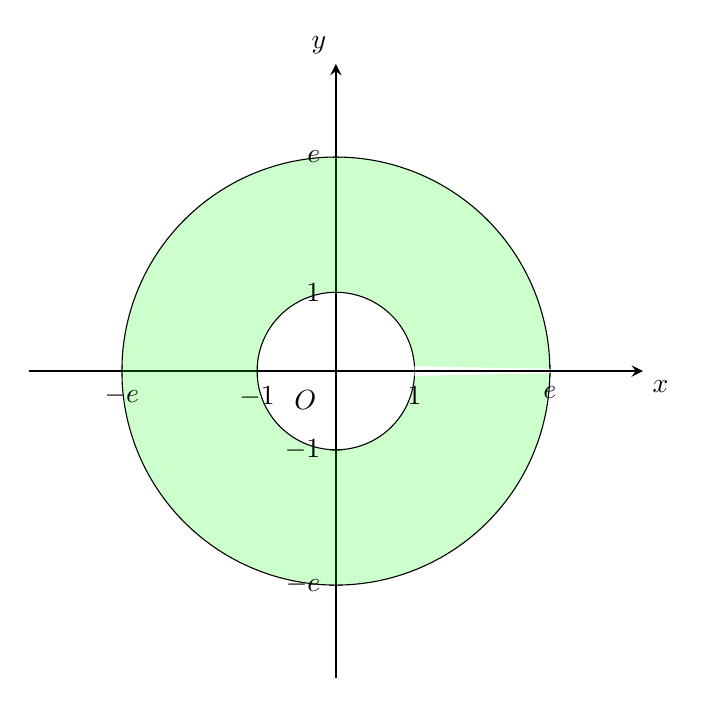
\begin{tikzpicture}
    \begin{axis}[standard,
            xtick={-2.718,-1,1,2.718},
            ytick={-2.718,-1,1,2.718},
            samples=1000,
            xlabel={$x$},
            ylabel={$y$},
            xmin=-3,xmax=3,
            ymin=-3,ymax=3,
            x=1cm,
            y=1cm/1,
            xticklabels={$-e$, $-1$, $1$, $e$},
            yticklabels={$-e$, $-1$, $1$, $e$}
           ]
\node[anchor=center,label=south west:$O$] at (axis cs:0,0){};
\addplot[name path=F,domain={-2.718:2.718}]{sqrt(2.718^2-x^2};
\addplot[name path=G,domain={-2.718:2.718}]{-sqrt(2.718^2-x^2};
\addplot[name path=H,domain={-1:1}]{sqrt(1-x^2)};
\addplot[name path=I,domain={-1:1}]{-sqrt(1-x^2)};
\addplot[fill=green, fill opacity=0.2] fill between [of=F and H, soft clip={domain=-2.718:2.718}];
\addplot[fill=green, fill opacity=0.2] fill between [of=G and I, soft clip={domain=-2.718:2.718}];
    \end{axis}
    \end{tikzpicture}
}
\end{center}
Based on the graph, it looks like our angle $\theta$ is between $0$ and $2\pi$.

We can get our lower bound of $r$ from the curve $1=x^2+y^2$.
\begin{align*}
    1&=x^2+y^2\\
    1&=r^2\tag{in polar, $x^2+y^2=r^2$}\\
    1&=r\tag{keep positive $r$}
\end{align*}
We can get our upper bound of $r$ from the curve $x^2+y^2=e^2$.
\begin{align*}
    x^2+y^2&=e^2\\
    r^2&=e^2\tag{in polar, $x^2+y^2=r^2$}\\
    r&=e\tag{keep positive $r$}
\end{align*}
Now, we can translate our Cartesian integral into its equivalent polar integral.
\begin{align*}
    \iint_R \frac{\ln(x^2+y^2)}{x^2+y^2}\,dA&=\int_0^{2\pi}\int_1^e \lrp{\frac{\ln (r^2)}{r^2}}r\,dr\,d\theta\tag{in polar, $x^2+y^2=r^2$}\\
   &= \int_0^{2\pi}\int_1^e\frac{\ln(r^2)}{r}\,dr\,d\theta\\
    &\int_0^{2\pi}\int_1^e\frac{2\ln r}{r}\,dr\,d\theta\\
    &=\int_0^{2\pi}\lrb{(\ln r)^2}_1^e\,d\theta\tag{u-sub}\\
    &=\int_0^{2\pi} 1^2 - 0^2 \,d\theta\\
    &=\int_0^{2\pi} 1 \,d\theta\\
    &=\lrb{\theta}_0^{2\pi}\\
    &=\boxed{2\pi}
\end{align*}
\textbf{Problem 3}

Evaluate the improper integral $\displaystyle \int_0^{\infty}\int_0^{\infty}\frac{1}{(1+x^2+y^2)^2}\,dx\,dy$

\Solution

It's a good idea to graph the Cartesian region to see how it would relate to the polar region. We will be graphing $0\leq x \leq \infty$ and $0\leq y \leq \infty$.
\begin{center}
\resizebox{3.5cm}{!}{
    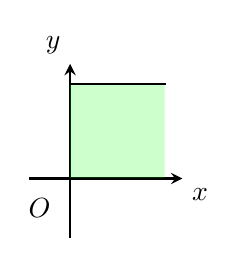
\begin{tikzpicture}
    \begin{axis}[standard,
            xtick={0},
            ytick={0},
            samples=1000,
            xlabel={$x$},
            ylabel={$y$},
            xmin=-0.3,xmax=1.2,
            ymin=-.5,ymax=1.2,
            x=1cm,
            y=1cm/1,
           ]
\node[anchor=center,label=south west:$O$] at (axis cs:0,0){};
\addplot[name path=F,domain={0:1.2}]{0};
\addplot[name path=G,domain={0:1.2}]{1.2};
\addplot[fill=green, fill opacity=0.2] fill between [of=F and G, soft clip={domain=0:1.2}];
    \end{axis}
    \end{tikzpicture}
}
\end{center}
Based on the graph, it looks like our angle $\theta$ is between $0$ and $\dfrac{\pi}{2}$. It also looks like our $r$ is between $0$ and $\infty$.

Now, we can translate our Cartesian integral into its equivalent polar integral.
\begin{align*}
    \int_0^{\infty}\int_0^{\infty}\frac{1}{(1+x^2+y^2)^2}\,dx\,dy&=\int_0^{\frac{\pi}{2}}\int_0^\infty \lrp{\frac{1}{(1+r^2)^2}}r\,dr\,d\theta\tag{in polar, $x^2+y^2=r^2$}\\
    &=\int_0^{\frac{\pi}{2}} \,d\theta \times \int_0^\infty \frac{r}{(1+r^2)^2}\,dr\tag{ok because $r$ is not a function of $\theta$}\\
    &=\lrb{\theta}_0^{\frac{\pi}{2}}\times \lrp{\lim_{t\to\infty}\int_0^t\frac{r}{(1+r^2)^2}\,dr}\\
    &=\frac{\pi}{2}\times\lrp{\lim_{t\to\infty}\frac{1}{2}\int_0^{t}\frac{1}{(1+u)^2}}\,du\\
    &=\frac{\pi}{2}\times\lrp{\lim_{t\to\infty}\frac{1}{2} \lrb{-(1+u)^{-1}}_0^t}\\
    &=\frac{\pi}{2}\times\lrp{\lim_{t\to\infty}\frac{1}{2}\lrp{-\frac{1}{1+t}+\frac{1}{1+0}}}\\
    &=\frac{\pi}{2}\times\lrp{\lim_{t\to\infty}-\frac{1}{2(1+t)}+\frac{1}{2}}\\
    &=\frac{\pi}{2}\times\lrp{0+\frac{1}{2}}\\
    &=\boxed{\frac{\pi}{4}}
\end{align*}
\textbf{Problem 4}

Use a double integral and polar coordinate to evaluate $\displaystyle I=\int_0^{\infty}e^{-x^2}\,dx$

\Solution

Following the hint, let's write 
\begin{align*}
    I^2=\lrp{\int_0^\infty e^{-x^2}\,dx}\lrp{\int_0^{\infty}e^{-y^2}\,dy}
\end{align*}
and then turn it into a double integral and convert to polar coordinates.
\begin{align*}
     I^2&=\lrp{\int_0^\infty e^{-x^2}\,dx}\lrp{\int_0^{\infty}e^{-y^2}\,dy}\\
     &=\int_0^{\infty}\int_0^{\infty}e^{-x^2}e^{-y^2}\,dx\,dy\tag{ok to combine since they're not functions of each other}\\
     &=\int_0^{\infty}\int_0^{\infty}e^{-(x^2+y^2)}\,dx\,dy
\end{align*}
It's a good idea to graph the Cartesian region to see how it would relate to the polar region. We will be graphing $0\leq x \leq \infty$ and $0\leq y \leq \infty$.
\begin{center}
\resizebox{3.5cm}{!}{
    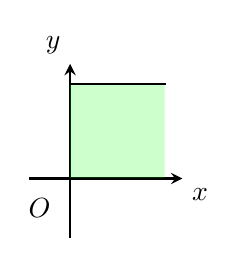
\begin{tikzpicture}
    \begin{axis}[standard,
            xtick={0},
            ytick={0},
            samples=1000,
            xlabel={$x$},
            ylabel={$y$},
            xmin=-0.3,xmax=1.2,
            ymin=-.5,ymax=1.2,
            x=1cm,
            y=1cm/1,
           ]
\node[anchor=center,label=south west:$O$] at (axis cs:0,0){};
\addplot[name path=F,domain={0:1.2}]{0};
\addplot[name path=G,domain={0:1.2}]{1.2};
\addplot[fill=green, fill opacity=0.2] fill between [of=F and G, soft clip={domain=0:1.2}];
    \end{axis}
    \end{tikzpicture}
}
\end{center}
Based on the graph, it looks like our angle $\theta$ is between $0$ and $\dfrac{\pi}{2}$. It also looks like our $r$ is between $0$ and $\infty$.

Now, we can translate our Cartesian integral into its equivalent polar integral.
\begin{align*}
    \int_0^{\infty}\int_0^{\infty}e^{-(x^2+y^2)}\,dx\,dy&=\int_0^{\frac{\pi}{2}}\int_0^\infty\lrp{ e^{-r^2}}r\,dr\,d\theta \tag{in polar $x^2+y^2=r^2$}\\
    &=\int_0^{\frac{\pi}{2}}\,d\theta\times\lrp{\lim_{t\to\infty}\int_0^t re^{-r^2}\,dr}\tag{ok because $r$ is not a function of $\theta$}\\
    &=\lrb{\theta}_0^{\frac{\pi}{2}}\times\lrp{\lim_{t\to\infty}\frac{1}{2}\int_0^t e^{-u}\,du}\tag{u sub, $u=r^2$}\\
    &=\frac{\pi}{2}\times\lrp{\lim_{t\to\infty}\frac{1}{2}\lrb{-e^{-u}}_0^t}\\
    &=\frac{\pi}{2}\times\lrp{\lim_{t\to\infty}-\frac{1}{2}e^{-t}+\frac{1}{2}}\\
    &=\frac{\pi}{2}\times\lrp{0+\frac{1}{2}}\\
    &={\frac{\pi}{4}}
\end{align*}
This is not our final answer! This is what $I^2$ is, not $I$. Our final answer is actually
\begin{align*}
    I^2&=\frac{\pi}{4}\\
    \alignedbox{I}{=\frac{\sqrt{\pi}}{2}}
\end{align*}
We keep the positive answer because graphically, the area under the graph of $\displaystyle \int_0^{\infty} e^{-x^2}\,dx$ is going to be a positive area.
\end{document}